During the anomaly propagation chain analysis process, we need to continuously detect whether a service is an anomalous service in terms of certain quality metrics.
For example, for the analysis process shown in Figure~\ref{fig:propagation}, we first identify $S_4$ and $S_7$ in entry node analysis and then $S_7$, $S_9$, and $S_{10}$ in anomaly propagation chain extension by service anomaly detection.
Given an upstream/downstream service $S'$ of the current service $S$, we detect possible anomaly with $S'$ in terms of different anomaly types by analyzing the historical data of the corresponding quality metrics (i.e., RT, EC, QPS) of the service call between $S'$ and $S$.
Based on the characteristics of different quality metrics, we choose a different analysis model for each anomaly type.
These analysis models are designed based on the characteristics of the fluctuations of the corresponding quality metrics as shown in Figure~\ref{fig:all-metrics}.
These data are obtained from the monitoring system of Alibaba.

%Aiming at different issues that affect the high availability of microservice system, \app~adopts different anomaly detection models according to different metrics characteristics and the actual situation of online fault data.
%It is mainly composed of reliability issue detection model, performance issue detection model and traffic issue detection model. The main methods used are Random Forest(RF), three-sigma rule of thumb(3Sigma), One-class Support Vector Machines(OC-SVM)\cite{ocsvm}.

\begin{figure*}[ht]
    \centering
    \subfigure[RT fluctuations in two hours]{
        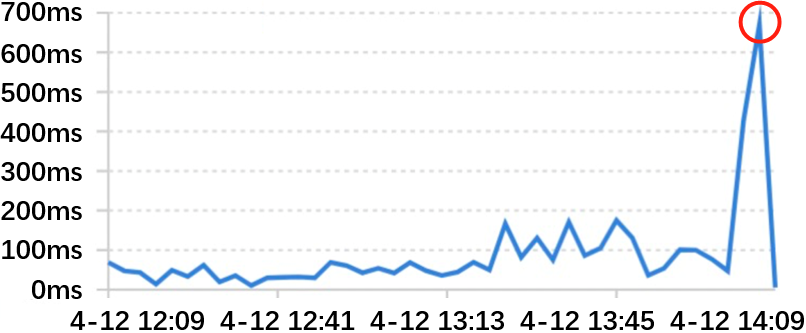
\includegraphics[width=5.5cm]{images/rt-hour.png}\label{fig:RT-2-hour}
    }
    \subfigure[EC fluctuations in two hours]{
        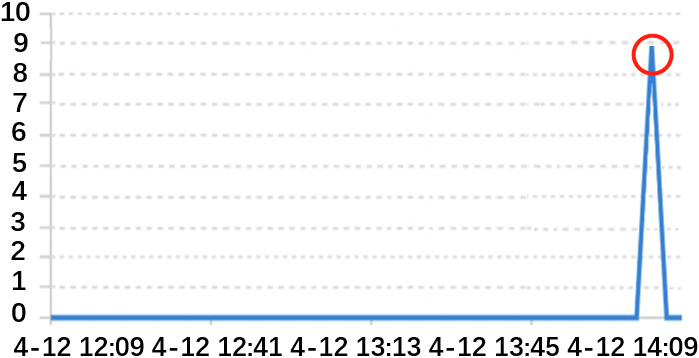
\includegraphics[width=5.5cm]{images/ec-hour.png}\label{fig:EC-2-hour}
    }
    \subfigure[QPS fluctuations in two hours]{
        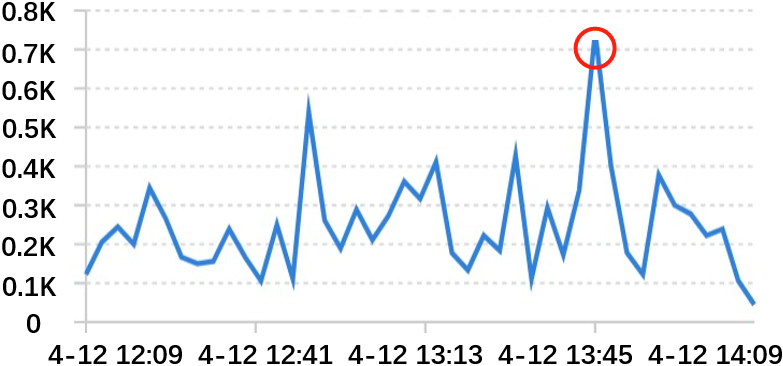
\includegraphics[width=5.5cm]{images/qps-hour.png}\label{fig:QPS-2-hour}
    }
    \quad
    \subfigure[RT fluctuations in one week]{
        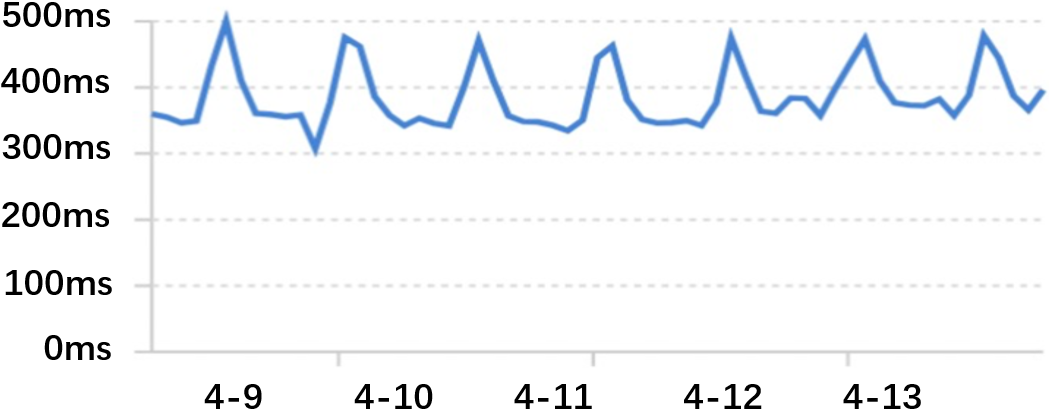
\includegraphics[width=5.5cm]{images/rt-week.png}\label{fig:RT-week}
    }
    \subfigure[EC fluctuations in one week]{
        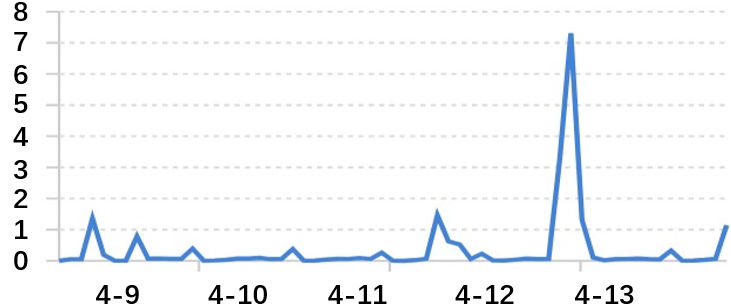
\includegraphics[width=5.5cm]{images/ec-week.png}\label{fig:EC-week}
    }
    \subfigure[QPS fluctuations in one week]{
        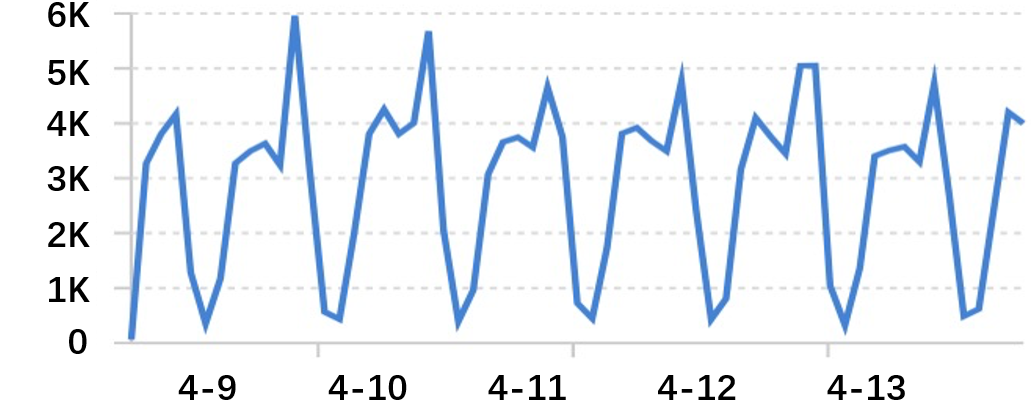
\includegraphics[width=5.5cm]{images/qps-week.png}\label{fig:QPS-week}
    }
    \quad
    \caption{Fluctuation of Quality Metrics}\label{fig:all-metrics}
\end{figure*}

\subsubsection{Performance Anomaly}
Performance anomaly is detected based on the anomalous increase of response time (RT).
The challenge here is how to distinguish anomalous fluctuations from normal fluctuations. 
Figure~\ref{fig:RT-2-hour} and Figure~\ref{fig:RT-week}  illustrate the fluctuations of response time in two hours and in one week respectively.
It can be seen that there are periodic fluctuations in different periods of a day and different days of a week.
If we use intuitive rules like 3-sigma, it is likely that some of these periodic fluctuations will be recognized as performance anomalies.
To recognize anomalous fluctuations such as the anomalous point in Figure~\ref{fig:RT-2-hour}, we need to consider not only the quality metrics of the current period but also those of the same period of the previous day and the same day of the previous week.
Moreover, in historical data the response time is in normal fluctuations most of the time, and there are only a few anomalous fluctuations.

Based on the characteristics of RT, we choose to use OC-SVM (one class support vector machine) to train a prediction model for anomalous RT fluctuations.
OC-SVM~\cite{ocsvm} uses only the information for the target class (normal RT fluctuations) to learn a classifier that can recognize the samples belonging to the target class and identify the others as outliers (anomalous RT fluctuations).
OC-SVM is known to have the advantages of simple modelling, strong interpretability, and better generalization ability than clustering methods.
We define and use the following four kinds of features for the model.

\begin{itemize}
\item \textbf{Number of Over-Max Values}: the number of RT values in the current detection window that exceed the maximum RT value of a given comparison period.

\item \textbf{Delta of Maximum Values}: the delta between the maximum RT value in the current detection window and the maximum RT value of a given comparison period.

\item \textbf{Number of Over-Average Values}: the number of RT values in the current detection window that exceed the maximum moving average of the RT values of a given comparison period.

\item \textbf{Ratio of Average Values}: the ratio of the average of the RT values in the current detection window to the maximum moving average of the RT values of a given comparison period.
\end{itemize}

We consider the last 10 minutes as the current detection window, i.e., considering the 10 RT values of the last 10 minutes.
For the comparison periods, we consider the following three settings: the last one hour before the current detection window, the same hour of the previous day, the same hour of the same day of the previous week.
Therefore, we have 12 features in total for the OC-SVM model.

We use the Python based machine learning framework scikit-learn~\cite{scikitLearn} to implement the model.
To train the model, we collect 100,000 cases of different services from the monitoring infrastructure of Alibaba.
Each case includes a series of RT values of the current detection window and different comparison periods.
We also collect 600 cases for verifying the trained model. 
These cases are different from the training cases and the ratio of positive and negative cases is 1:1.
The results of the verification are shown in Table~\ref{tab:performance_train}, which provide the recall, precision,
F1-measure, FPR (False Positive Rate) of performance anomaly detection with different coverage of the training set.
It can be seen that the model can accurately detect performance anomalies with only 10-20\% of the training set, and it can achieve very high accuracy when using 70\% of the training set.

\begin{table}[ht]
	\newcommand{\tabincell}[2]{\begin{tabular}{@{}#1@{}}#2\end{tabular}}
	\caption{Accuracy of Performance Anomaly Detection}
	\label{tab:performance_train}
    \small
	\centering
	%\resizebox{0.48\textwidth}{!}{
		\begin{tabular}{|c|c|c|c|c|}
			\hline \textbf{Coverage} & \textbf{Recall} & \textbf{Precision} & \textbf{F1} & \textbf{FPR}\\
			\hline 10\%  &  0.86 & 0.73 & 0.79 & 0.32 \\
			\hline 20\%  &  0.81 & 0.88 & 0.84 & 0.12 \\
            \hline 30\%  &  0.82 & 0.92 & 0.87 & 0.07 \\
			\hline 40\%  &  0.83 & 0.92 & 0.87 & 0.08 \\
			\hline 50\%  &  0.84 & 0.94 & 0.89 & 0.06 \\
            \hline 60\%  &  0.83 & 0.94 & 0.88 & 0.06 \\
			\hline 70\%  &  0.86 & 0.95 & 0.90 & 0.05 \\
			\hline 80\%  &  0.87 & 0.95 & 0.91 & 0.05 \\
            \hline 90\%  &  0.87 & 0.95 & 0.91 & 0.04 \\
            \hline 100\% &  0.87 & 0.96 & 0.91 & 0.03 \\
			\hline
		\end{tabular}
	%}
	\vspace{-3pt}
\end{table}



\subsubsection{Reliability Anomaly}
Reliability anomaly is detected based on the anomalous increase of error counts (EC).
As shown in Figure~\ref{fig:EC-2-hour} and Figure~\ref{fig:EC-week}, the value of EC is 0 most of the time.
In some cases, even when some errors are raised there is no influence on the business and the service may get back to normal in a short time.
For example, service calls fail and errors are raised when the circuit break is open, but the service will get back to normal soon after the load decreases and the circuit break is closed.
Therefore, we cannot use the performance anomaly detection model to detect reliability anomalies.
Binary classification models like Logic Regression (LR) or Random Forest (RF) can be used.
However, as only a small number of EC changes are reliability anomalies, LR models are likely to cause overfitting.

Based on the characteristics of EC, we choose to use Random Forest (RF) to train a prediction model for anomalous EC increases.
RF uses multiple decision trees for classification.
It can effectively combine multiple features and avoid overfitting.
We define and use the following five features for the model.
Note that some of the features combine other metrics (e.g., RT, QPS) together with EC, as anomalous EC increases often correlate with RT and QPS.
Similar to performance anomaly detection, we consider the last 10 minutes as the current detection window.

%At the same time, we use RT in reliability anomaly detection, because we found that in the actual system RT and EC are related, for example an interface response timeout anomaly may cause timeout exception information in the log.
%We use Threshold and Correlation to reflect the relationship between RT and EC.
%In the otherwise, we use MaxErrorRate that calculated by QPS and EC to reflect the maximum error rate in the detection window.

\begin{itemize}
\item \textbf{Previous Day Delta Outlier Value}: calculate the deltas of the EC values in the last one hour and the EC values in the same hour of the previous day; use the 3-sigma rule to identify possible outliers of the deltas in the current detection window; if exist return the average of the outliers as the feature value, otherwise return 0.

\item \textbf{Previous Minute Delta Outlier Value}: 
calculate the deltas of the EC values and the values of the previous minute in the last one hour; 
use the 3-sigma rule to identify possible outliers of the deltas in the current detection window; 
if exist return the average of the outliers as the feature value, otherwise return 0.

\item \textbf{Response Time Over Threshold}: whether the average RT in the current detection window exceeds a predefined threshold (e.g., 50ms).

\item \textbf{Maximum Error Rate}: the maximum error rate (i.e., EC divided by number of requests) in the current detection window.

\item \textbf{Correlation with Response Time}: the Pearson correlation coefficient (see Equation~\ref{eq:pearson}) between EC and RT in the current detection window.

\end{itemize}

We use the Python based machine learning framework scikit-learn~\cite{scikitLearn} to implement the model.
To train the model, we collect 1,000 labelled cases of different services from the monitoring infrastructure of Alibaba and the ratio of positive and negative samples is 1:3.
We also collect 400 cases for verifying the trained model and the ratio of positive and negative samples is 5:3.
The results of the verification are shown in Table~\ref{tab:reliability_train}, which provide the recall, precision,
F1-measure, FPR (False Positive Rate) of reliability anomaly detection with different coverage of the training set.
It can be seen that the model can accurately detect reliability anomalies with only 20\% of the training set, and it can achieve very high accuracy when using 40\% of the training set.

\begin{table}[ht]
	\newcommand{\tabincell}[2]{\begin{tabular}{@{}#1@{}}#2\end{tabular}}
	\caption{Accuracy of Reliability Anomaly Detection}
	\label{tab:reliability_train}
    \small
	\centering
		\begin{tabular}{|c|c|c|c|c|}
			\hline \textbf{Coverage} & \textbf{Recall} & \textbf{Precision} & \textbf{F1} & \textbf{FPR}\\
			\hline 10\%  &  0.29 & 1    & 0.44 & 0.70 \\
			\hline 20\%  &  0.64 & 1    & 0.78 & 0.35 \\
            \hline 30\%  &  0.64 & 1    & 0.78 & 0.35 \\
			\hline 40\%  &  0.86 & 0.97 & 0.91 & 0.14 \\
			\hline 50\%  &  0.88 & 0.95 & 0.91 & 0.12 \\
            \hline 60\%  &  0.88 & 0.90 & 0.89 & 0.12 \\
			\hline 70\%  &  0.93 & 0.90 & 0.92 & 0.09 \\
			\hline 80\%  &  0.95 & 0.95 & 0.94 & 0.07 \\
            \hline 90\%  &  0.95 & 0.95 & 0.95 & 0.04 \\
            \hline 100\% &  0.98 & 0.93 & 0.95 & 0.02 \\
			\hline
		\end{tabular}
	\vspace{-3pt}
\end{table}



\subsubsection{Traffic Anomaly}
Traffic anomaly is detected based on the anomalous fluctuations of queries per second (QPS).
As shown in Figure~\ref{fig:QPS-2-hour} and Figure~\ref{fig:QPS-week}, QPS complies with the normal distribution in both short term and long term.
Therefore, we choose to use the 3-sigma rule to detect anomalous QPS fluctuations.

Similar to performance and reliability anomaly detection, we consider the last 10 minutes as the current detection window.
Based on the QPS values in the last one hour, we use the 3-sigma rule to detect outliers in the current detection window.
To further eliminate false positives, we also check the Pearson correlation coefficient (see Equation~\ref{eq:pearson}) between the QPS values and the business metric values of the initial anomalous service.
Only when the correlation is higher than a predefined threshold (e.g., 0.9) and  3-sigma outliers are identified in the current detection window, a traffic anomaly is reported for the current service.

%\begin{figure}[ht]
%	\centering
%	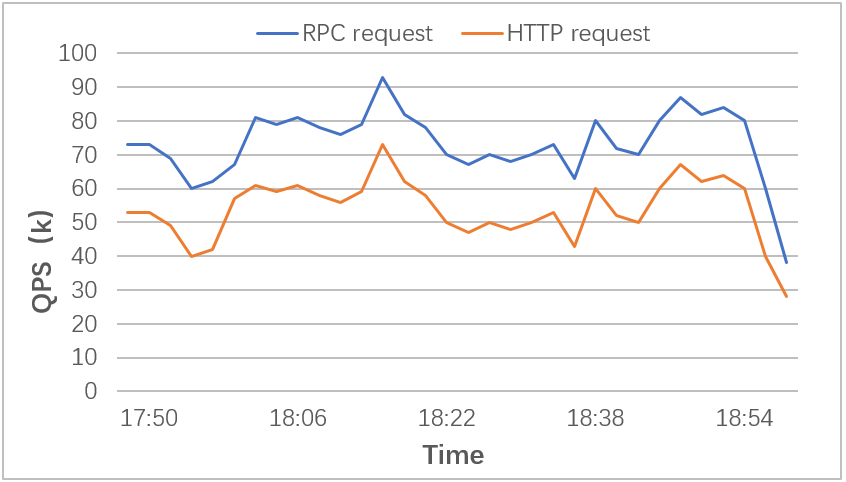
\includegraphics[width=0.45\textwidth]{images/qps-time.png}
%	\vspace{-8pt}
%	\caption{Change of QPS Over Time}\label{fig:qps-time}
%	\vspace{-10pt}
%\end{figure}



